%%%%%%%%%%%%%%%%%%%%%%%%%%%%%%%%%%%%%%%%%%%%%%%%%%%%%%%%%%%%%%%%%%%%%%%%%%%%%%%
\section{Data flow examples}
%%%%%%%%%%%%%%%%%%%%%%%%%%%%%%%%%%%%%%%%%%%%%%%%%%%%%%%%%%%%%%%%%%%%%%%%%%%%%%%
% %%%%%%%%%%%%%%%%%%%%%%%%%%%%%%%%%%%%%%%%%%%%%%%%%%%%%%%%%%%%%%%%%%%%%%%%%%%%%%%
% \subsection{Blocked matrix multiplication}
% %------------------------------------------------------------------------------
% \begin{frame}[plain,fragile]
%   \frametitle{Blocked matrix multiplication}
% \begin{block}{}
% \begin{lstlisting}[language=]
% for( i = 0; i < NB; i++ )
%     for( j = 0; j < NB; j++ )
%         for( k = 0; k < NB; k++ )
%             GEMM( A(i, k), A(k, j), A(i, j) );
% \end{lstlisting}
% \end{block}
% \end{frame}
% %------------------------------------------------------------------------------
% \begin{frame}[plain,fragile]
%   \frametitle{OmpSs}
% \begin{block}{}
% \begin{lstlisting}[basicstyle=\scriptsize\ttfamily]
% #pragma omp target device (smp) 
% #pragma omp task in([BS*BS]A, [BS*BS]B) inout([BS*BS]C)
% void matmul_tile(float *A, float *B, float *C, int BS) {
%   cblas_dgemm(CblasRowMajor, CblasNoTrans, CblasNoTrans,
%        BS, BS, BS, 1.0, A, BS, B, BS, 1.0, C, BS);
% }
% 
% void matmul(int mb, int nb, int kb,
%                           float **A, float **B, float **C, int BS) { 
%   int i, j, k;
%   for(i = 0; i < mb; i++)
%       for(j = 0; j < nb; j++)
%         for(k = 0; k < kb; k++)
%           matmul_tile(A[i*mb+k], B[k*kb+j], C[i*mb+j], BS);
% }
% \end{lstlisting}
% \end{block}
% \end{frame}
% %------------------------------------------------------------------------------
% \begin{frame}[plain,fragile]
%   \frametitle{StarPU}
% \begin{block}{}
% \begin{lstlisting}[basicstyle=\scriptsize\ttfamily]
% \end{lstlisting}
% \end{block}
% \end{frame}
% %------------------------------------------------------------------------------
% \begin{frame}[plain,fragile]
%   \frametitle{XKaapi}
% \begin{block}{}
% \begin{lstlisting}[basicstyle=\scriptsize\ttfamily]
% \end{lstlisting}
% \end{block}
% \end{frame}
% %------------------------------------------------------------------------------
%%%%%%%%%%%%%%%%%%%%%%%%%%%%%%%%%%%%%%%%%%%%%%%%%%%%%%%%%%%%%%%%%%%%%%%%%%%%%%%
\subsection{Tiled Cholesky factorization}
%------------------------------------------------------------------------------
\begin{frame}[plain,fragile]
  \frametitle{Tiled Cholesky factorization}
  \begin{itemize}
  \item Parallel algorithm from PLASMA [UTK].
  \end{itemize}
\begin{block}{}
\begin{lstlisting}[language=]
for( k = 0; k < NB; k++ ) {
    POTRF( A(k, k) );
    
    for( m = k+1; m < NB; m++ ){
        TRSM( A(k, k), A(m, k) );
    }

    for( m = k+1; m < NB; m++ ){
        SYRK( A(m, k), A(m, m) );

        for( n = k+1; n < m; n++ ){
           GEMM( A(m, k), A(n, k), A(m, n) );
	}
    }
}
\end{lstlisting}
\end{block}
\end{frame}
%------------------------------------------------------------------------------
\begin{frame}[plain,fragile]
  \frametitle{XKaapi}
  \vspace{-4mm}
  %
  \begin{block}{}
\begin{lstlisting}[basicstyle=\scriptsize\ttfamily]
struct TaskPOTRF: public ka::Task<3>::Signature
<
  CBLAS_ORDER,			      /* row / col */
  CBLAS_UPLO,             /* upper / lower */
  ka::RW<ka::range2d<double> > /* A */
>{};

struct TaskGEMM: public ka::Task<8>::Signature
<
  CBLAS_ORDER,			      /* row / col */
  CBLAS_TRANSPOSE,        /* NoTrans/Trans for A */
  CBLAS_TRANSPOSE,        /* NoTrans/Trans for B */
  double,                      /* alpha */
  ka::R<ka::range2d<double> >, /* Aik   */
  ka::R<ka::range2d<double> >, /* Akj   */
  double,                      /* beta */
  ka::RW<ka::range2d<double> > /* Aij   */
>{};
\end{lstlisting}
  \end{block}
\end{frame}
%------------------------------------------------------------------------------
\begin{frame}[plain,fragile]
  \frametitle{XKaapi}
  \vspace{-4mm}
\begin{block}{}
\begin{lstlisting}[basicstyle=\scriptsize\ttfamily]
struct TaskCholesky: public ka::Task<2>::Signature< ka::RPWP<ka::range2d<double> >, CBLAS_UPLO >{};

template<> struct TaskBodyCPU<TaskCholesky> {
  void operator()( ka::range2d_rpwp<double> A, const CBLAS_UPLO uplo)
  {
    size_t N = A->dim(0);
    size_t blocsize = global_blocsize;
    
    for (size_t k=0; k < N; k += blocsize) {
      ka::rangeindex rk(k, k+blocsize);
      ka::Spawn<TaskPOTRF>() ( A(rk,rk) );
      
      for (size_t m=k+blocsize; m < N; m += blocsize) {
        ka::rangeindex rm(m, m+blocsize);
        ka::Spawn<TaskTRSM>() (  A(rk,rk), A(rk,rm) );
      }
      
      for (size_t m=k+blocsize; m < N; m += blocsize) {
        ka::rangeindex rm(m, m+blocsize);
        ka::Spawn<TaskSYRK>() ( A(rk,rm), A(rm,rm) );
	
        for (size_t n=k+blocsize; n < m; n += blocsize) {
          ka::rangeindex rn(n, n+blocsize);
          ka::Spawn<TaskGEMM>() (  A(rk,rm), A(rk,rn), A(rn,rm) );
        }
      }
    }
  }
};
\end{lstlisting}
\end{block}
\end{frame}
%------------------------------------------------------------------------------
%\begin{frame}[plain,fragile]
%  \frametitle{XKaapi}
%\begin{block}{}
%\begin{lstlisting}[basicstyle=\scriptsize\ttfamily]
%\end{lstlisting}
%\end{block}
%\end{frame}
%------------------------------------------------------------------------------
\begin{frame}[plain]
  \frametitle{XKaapi data flow graph}
  \vspace*{-5mm}
  \begin{figure}[ht]
  \centering
  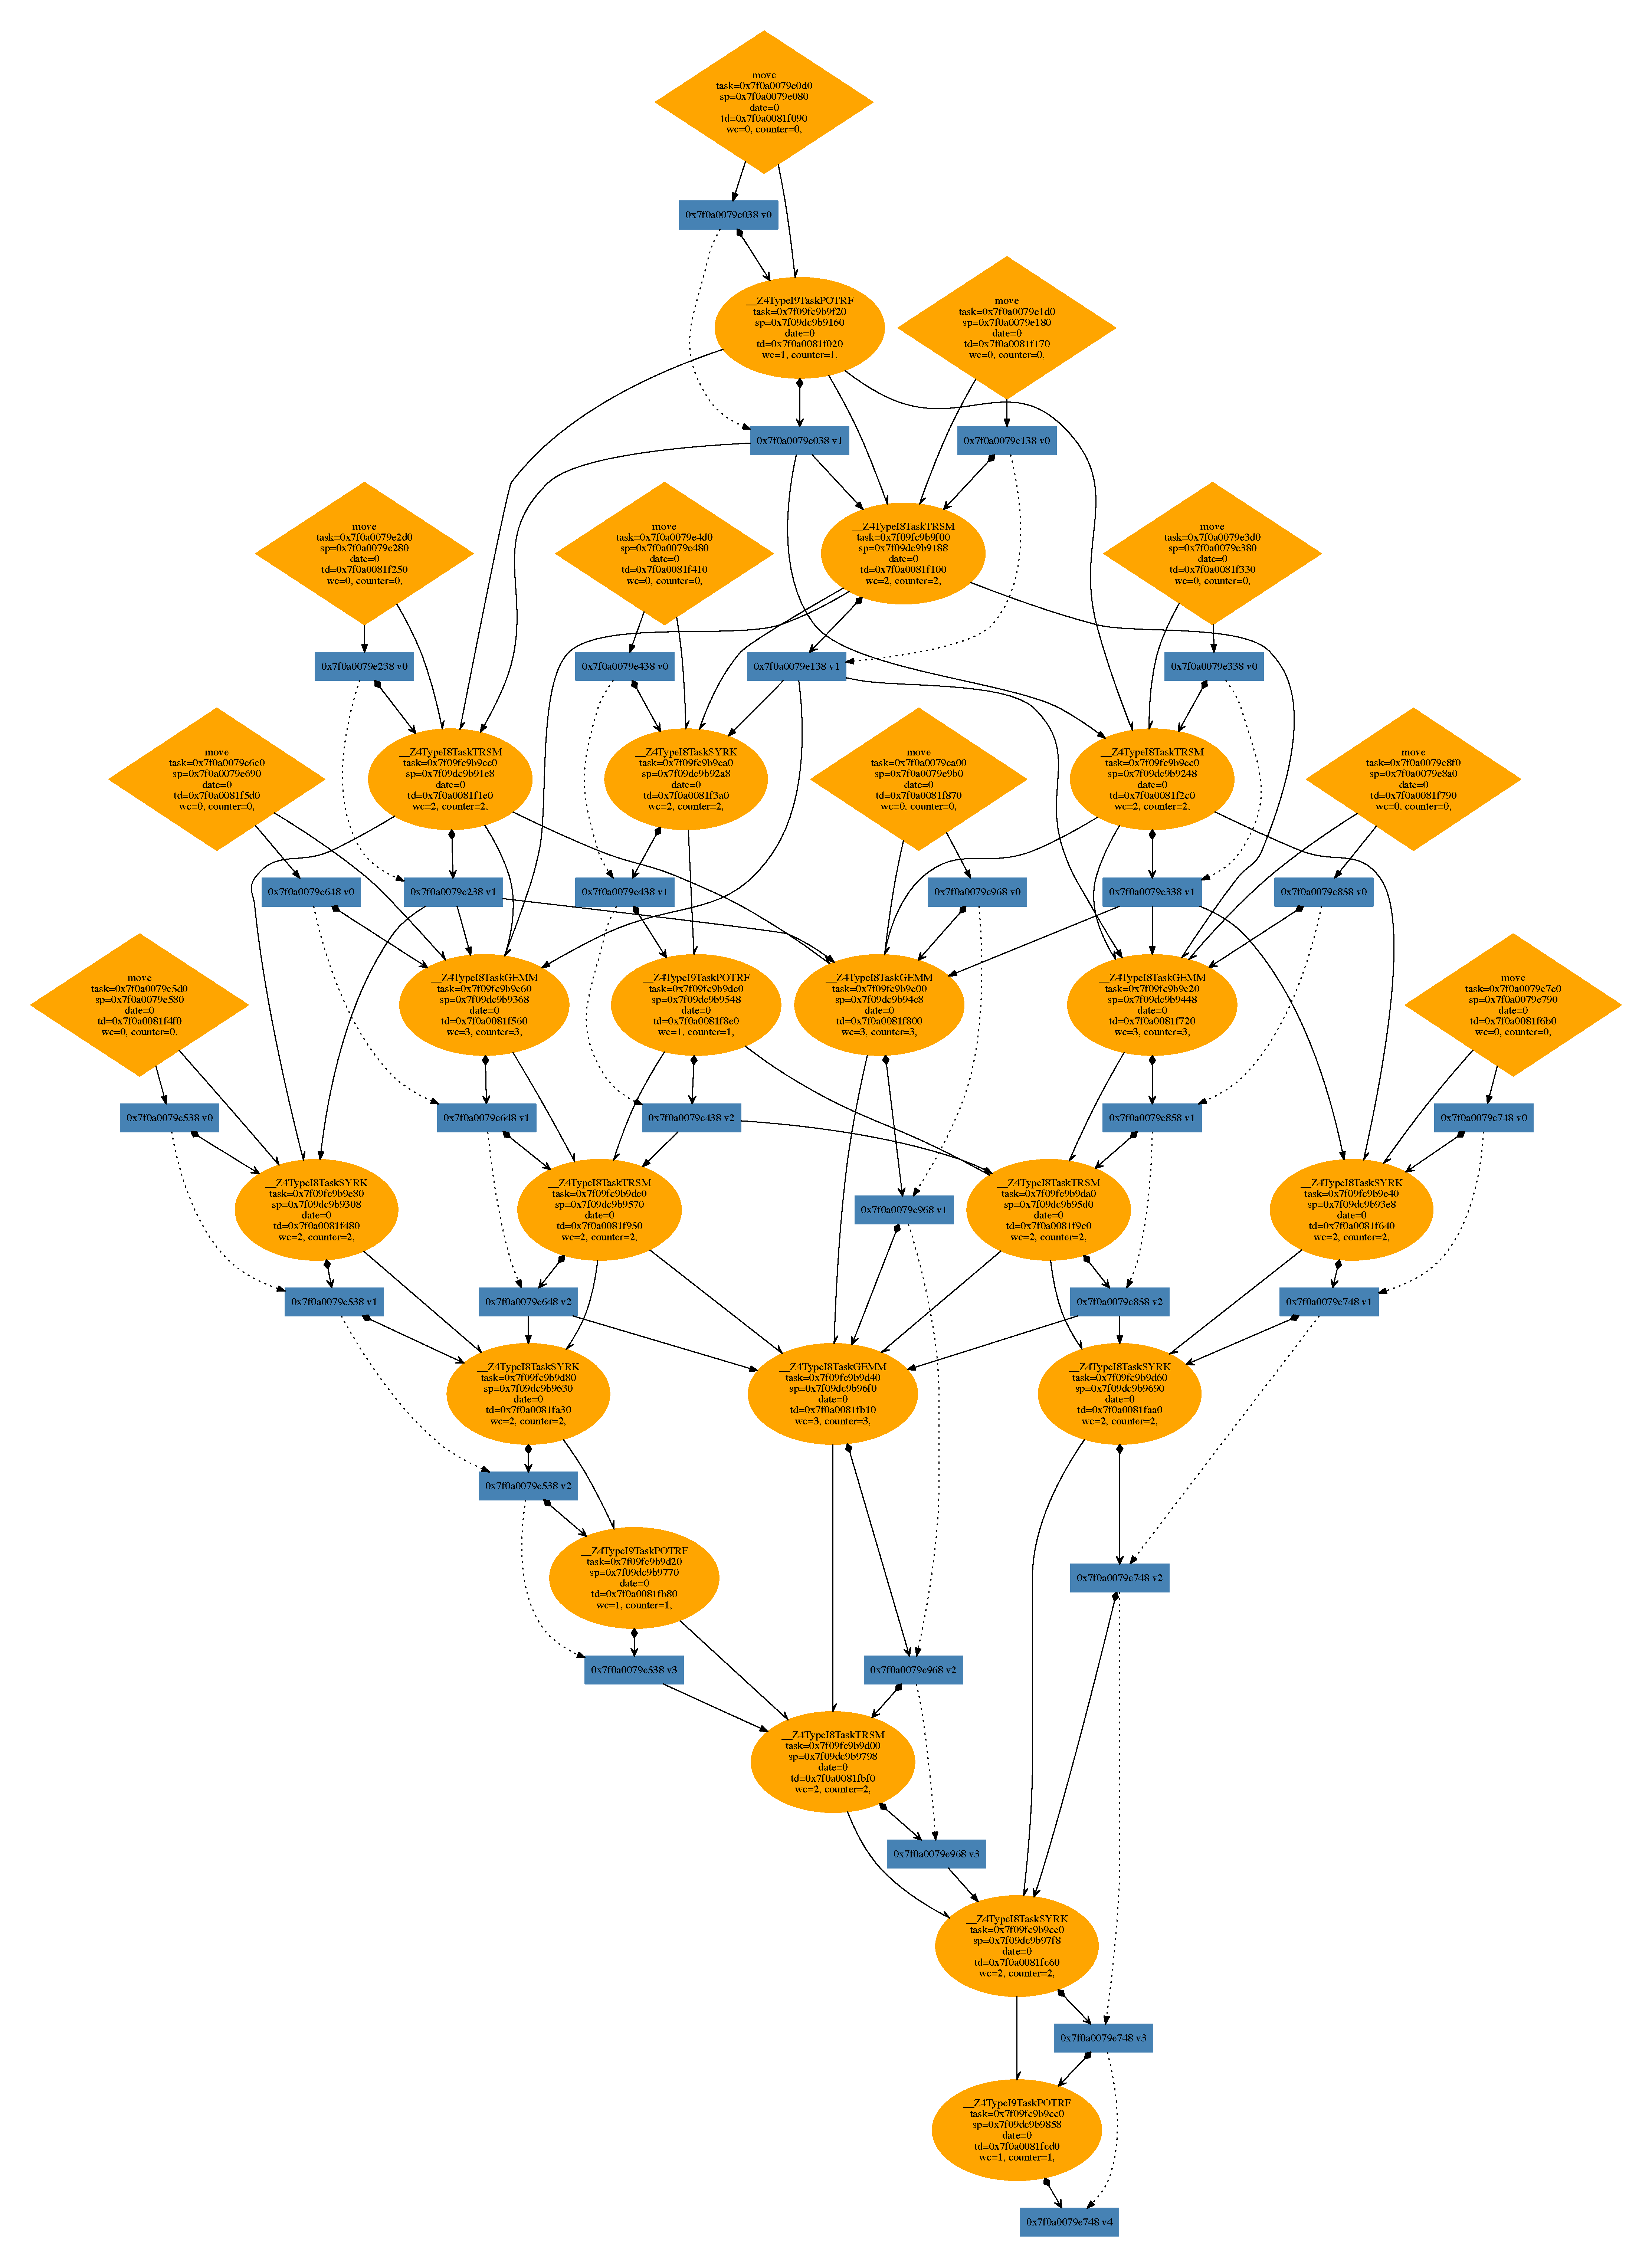
\includegraphics[width=0.5\textwidth]{chol-4096-1024}
  \end{figure}
\end{frame}
%------------------------------------------------------------------------------
\begin{frame}[plain,fragile]
  \frametitle{StarPU}
  \vspace{-4mm}
  %
  \begin{block}{}
\begin{lstlisting}[basicstyle=\scriptsize\ttfamily]
static struct starpu_codelet cl_dpotrf = {
    .modes = { STARPU_RW },
    .type = STARPU_SEQ,
    .where = STARPU_CPU,
    .cpu_funcs = {chol_cpu_codelet_update_dpotrf, NULL},
    .nbuffers = 1
};

static struct starpu_codelet cl_dtrsm = {
    .modes = { STARPU_R, STARPU_RW },
    .type = STARPU_SEQ,
    .where = STARPU_CPU,
    .cpu_funcs = {chol_cpu_codelet_update_dtrsm, NULL},
    .nbuffers = 2
};

static struct starpu_codelet cl_dsyrk = {
    .modes = { STARPU_R, STARPU_RW },
    .type = STARPU_SEQ,
    .where = STARPU_CPU,
    .cpu_funcs = {chol_cpu_codelet_update_dsyrk, NULL},
    .nbuffers = 2
};

static struct starpu_codelet cl_dgemm = {
    .modes = { STARPU_R, STARPU_R, STARPU_RW },
    .type = STARPU_SEQ,
    .where = STARPU_CPU,
    .cpu_funcs = {chol_cpu_codelet_update_dgemm, NULL},
    .nbuffers = 3
};
\end{lstlisting}
  \end{block}
\end{frame}
%------------------------------------------------------------------------------
\begin{frame}[plain,fragile]
  \frametitle{StarPU}
  \vspace{-4mm}
  %
  \begin{block}{}
\begin{lstlisting}[basicstyle=\scriptsize\ttfamily]
#define A(x,y)	    (dataA[nb*x+y])
static int cholesky( starpu_data_handle_t* dataA, unsigned N, unsigned nb ) {
    unsigned m, n, k;
    for (k = 0; k < nb; k++) {
        starpu_insert_task( &cl_dpotrf,
            STARPU_RW, A(k,k), 0);

        for (m = k+1; m < nb; m++) {
            starpu_insert_task( &cl_dtrsm,
                STARPU_R, A(k,k), STARPU_RW, A(m,k), 0);
        }

        for (m = k+1; m < nb; m++) {
            starpu_insert_task( &cl_dsyrk,
                STARPU_R, A(m,k), STARPU_RW, A(m,m), 0);

           for (n = k+1; n < m; n++){
               starpu_insert_task( &cl_dgemm,
                   STARPU_R, A(m,k), STARPU_R, A(n,k), STARPU_RW, A(m,n), 0);
	    }
      }
    }

    starpu_task_wait_for_all();
    return 0;
}
\end{lstlisting}
  \end{block}
\end{frame}
%------------------------------------------------------------------------------
%\begin{frame}[plain,fragile]
%  \frametitle{StarPU}
%  \vspace{-4mm}
%  %
%  \begin{block}{}
%\begin{lstlisting}[basicstyle=\scriptsize\ttfamily]
%\end{lstlisting}
%  \end{block}
%\end{frame}
%------------------------------------------------------------------------------
\begin{frame}[plain,fragile]
  \frametitle{OmpSs}
  \vspace{-4mm}
  %
  \begin{block}{}
\begin{lstlisting}[basicstyle=\scriptsize\ttfamily]
#pragma omp task inout([ts][ts]A)
void omp_potrf(double * const A, int ts, int ld) { /*  */ }

#pragma omp task in([ts][ts]A) inout([ts][ts]B)
void omp_trsm(double *A, double *B, int ts, int ld) { /*  */ }

#pragma omp task in([ts][ts]A) inout([ts][ts]B)
void omp_syrk(double *A, double *B, int ts, int ld) { /*  */ }

#pragma omp task in([ts][ts]A, [ts][ts]B) inout([ts][ts]C)
void omp_gemm(double *A, double *B, double *C, int ts, int ld) { /*  */ }

void cholesky_blocked(const int ts, const int nt, double* Ah[nt][nt])
{
   for (int k = 0; k < nt; k++) {
      omp_potrf (Ah[k][k], ts, ts);
      for (int i = k + 1; i < nt; i++) {
         omp_trsm (Ah[k][k], Ah[k][i], ts, ts);
      }
      for (int i = k + 1; i < nt; i++) {
         for (int j = k + 1; j < i; j++) {
            omp_gemm (Ah[k][i], Ah[k][j], Ah[j][i], ts, ts);
         }
         omp_syrk (Ah[k][i], Ah[i][i], ts, ts);
      }

   }
#pragma omp taskwait
}
\end{lstlisting}
  \end{block}
\end{frame}
%------------------------------------------------------------------------------
%%%%%%%%%%%%%%%%%%%%%%%%%%%%%%%%%%%%%%%%%%%%%%%%%%%%%%%%%%%%%%%%%%%%%%%%%%%%%%%
\subsection{Parallel SPMV}
%------------------------------------------------------------------------------
\begin{frame}[plain,fragile]
  \frametitle{Parallel SPMV}
  \begin{block}{}
\begin{lstlisting}[basicstyle=\scriptsize\ttfamily]
struct TaskParallelSPMV: public ka::Task<4>::Signature<
  float,			  /* alpha */
  ka::R<ka::range2d<float> >,	  /* A */
  ka::R<ka::range1d<float> >,	  /* x */
  ka::RPWP<ka::range1d<float> >	  /* y */
>{};

template<>
struct TaskBodyCPU<TaskParallelSPMV> {
  void operator()( float alpha, ka::range2d_r<float> A, ka::range1d_r<float> x,
         ka::range1d_rpwp<float> y )
  {
    int m = A->dim(0);
    int bloc = BLOCSIZE;
    float* const px = (float*)x.begin();
    float* const py = (float*)y.begin();
    
    for(int i=0; i < m; i += bloc)
    {
      ka::rangeindex ri(i, i+bloc);
      ka::range1d<float> rx(px, x.size());
      ka::range1d<float> ry(py+i, bloc);
     // In A, lines from i to i+bloc, entire column 
      ka::Spawn<TaskSPMV>()( alpha, A(ri, ka::rangeindex::full), rx, ry );
    }
  }
};
\end{lstlisting}
  \end{block}
\end{frame}
%------------------------------------------------------------------------------
\begin{frame}[plain]
  \frametitle{SPMV data flow graph}
%  \vspace*{-5mm}
  \begin{figure}[ht]
  \centering
  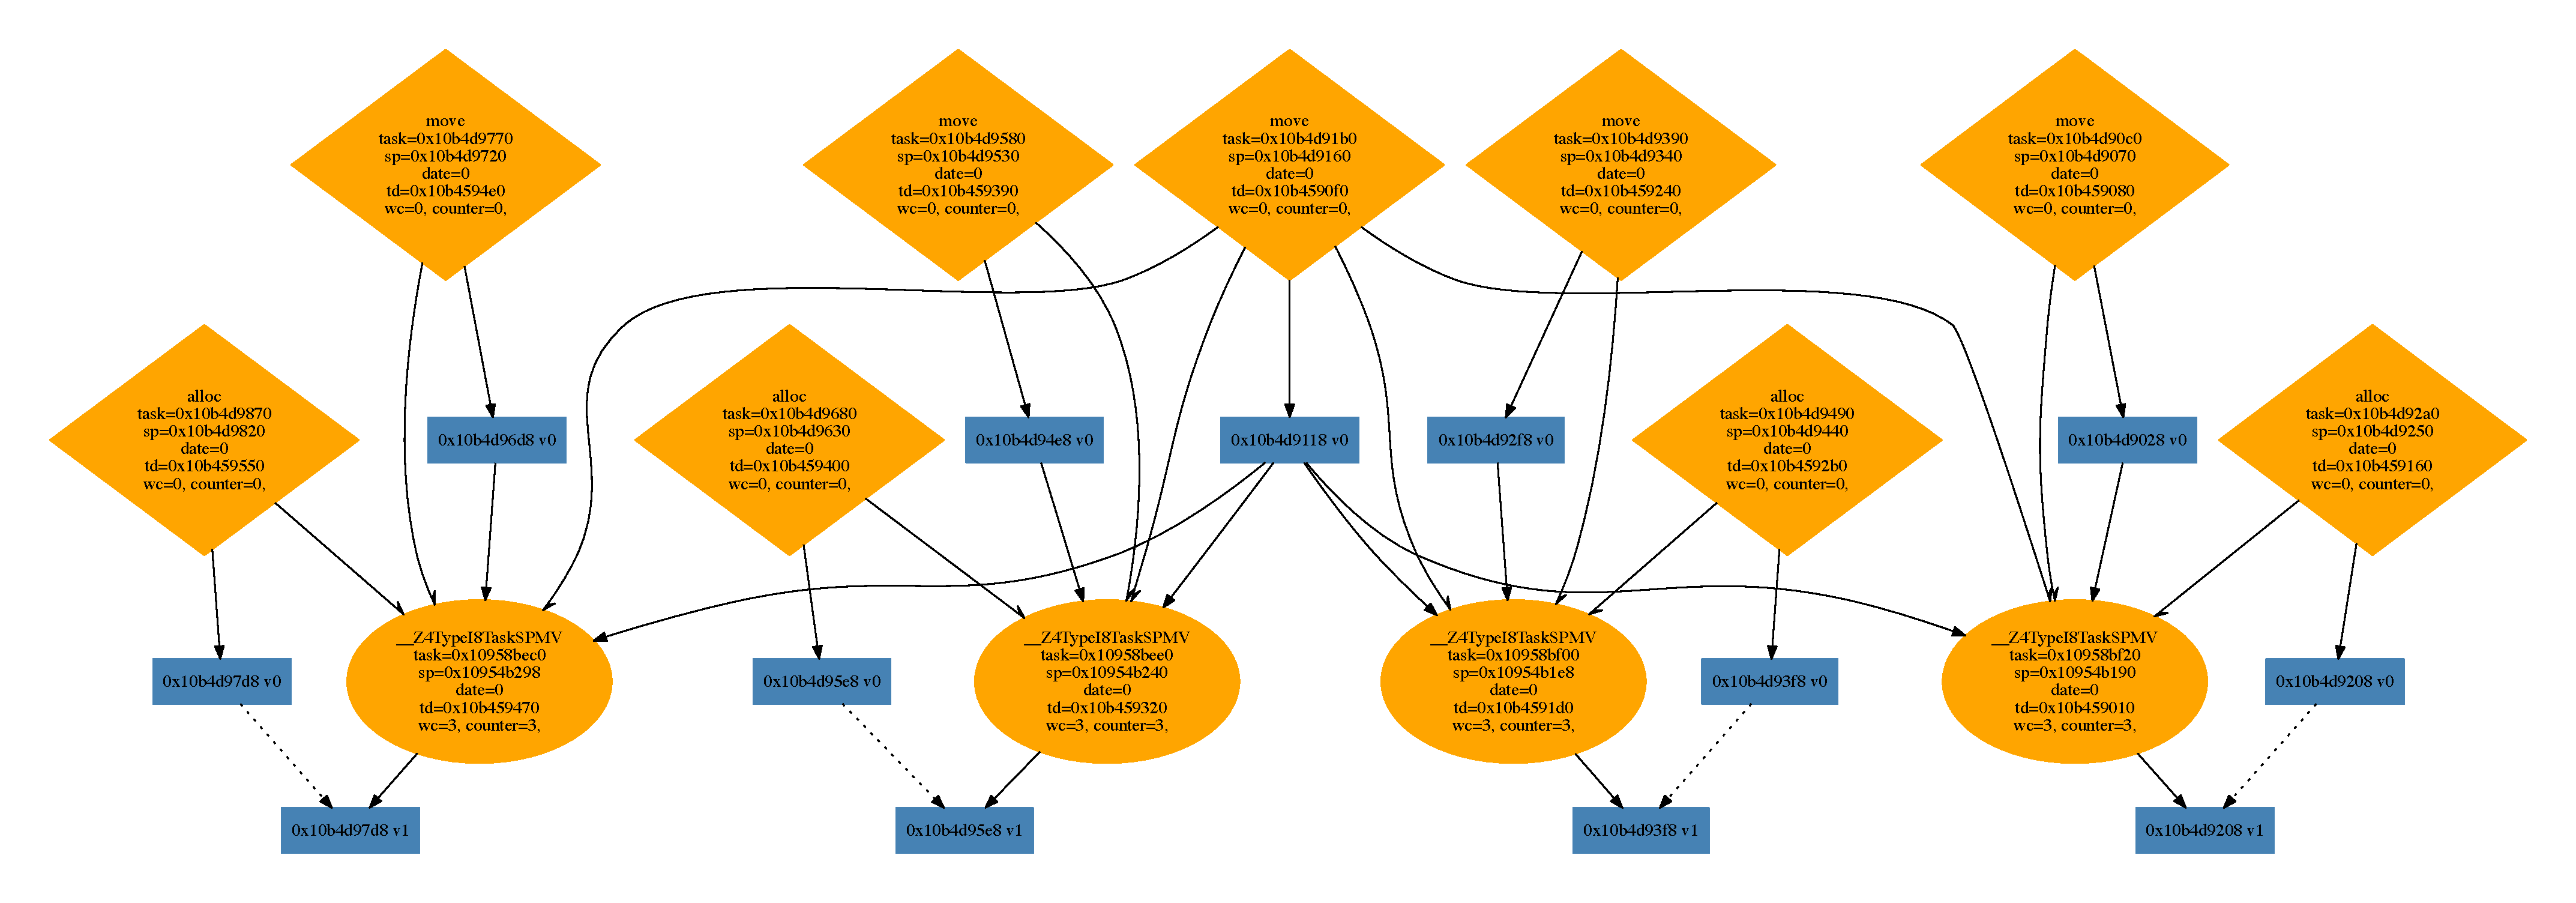
\includegraphics[width=\textwidth]{spmv-2048-512}
  \end{figure}
\end{frame}
%------------------------------------------------------------------------------
